%This is the fourth chapter of the dissertation

%The following command starts your chapter. If you want different titles used in your ToC and at the top of the page throughout the chapter, you can specify those values here. Since Columbia doesn't want extra information in the headers and footers, the "Top of Page Title" value won't actually appear.

\pagestyle{cu}
\graphicspath{{./AppendixA/images/}}

\chapter[GPUs and Fast Monte Carlo Matching for Parameter Estimation][GPUs and Fast Monte Carlo Matching for Parameter Estimation]{GPUs and Fast Monte Carlo Matching for Parameter Estimation}
\label{app:gpus}

In this appendix we will go into more detail about the analysis framework that was briefly mentioned in the previous chapters that was used for the electronic and nuclear recoil calibrations.  This framework, proposed and developed by the author for the analysis discussed in chapter four, enables the use of non-analytical models for parameter estimation in a reasonable time frame.  



\section{Motivation}

Oftentimes in physics, very complicated processes can be very well approximated by simple and analytical probability distributions.  There are many examples of these useful approximations in this work alone, including the majority of the calibrations for XENON1T (\secref{sec:xe1t_calibrations}) and neriX (\secref{sec:nerix_cals}).

However, the work in this appendix is an answer proposed by the author to the question of what do we do when no such approximation exists or is not appropriate?  This situation arises several times in this work: for the electronic and nuclear recoil calibration in XENON1T (\secref{sec:xe1t_er_nr_calibration}), the measurement of the nuclear recoil response of liquid xenon in neriX (\secref{sec:nerix_analysis}), and the characterization of the single photoelectron response of the neriX and XENON1T photomultiplier tubes (\appref{app:pmts}).


\section{Parameter Estimation through Monte Carlo}

\subsection{Overview}

For parameter estimation, the ultimate requirement is that you have a likelihood function that can be used to compare different sets of parameters with each other.  Many models are well approximated by an analytical distribution, such as a normal, Poisson, or exponential distribution to name a few of the most common.  When this is the case there are several common approaches to assigning a likelihood function.  One simple solution is to use the probability distribution function (PDF) of the distribution with the parameters under test evaluated at all points as the likelihood function, as shown in \eqnref{eqn:gpu_unbinned_likelihood} where $m$ is indexed over all of the data points.  Another approach is to use a binned likelihood, as shown in \eqnref{eqn:gpu_binned_likelihood} where $i$ is indexed over each of the bins, where we use the PDF to estimate the expected number of events in a given bin. 


\begin{equation}
        \label{eqn:gpu_unbinned_likelihood}
        \mathcal{L} = \prod_m f(\vec{x}_m; \vec{\theta})
\end{equation}

\begin{equation}
        \label{eqn:gpu_binned_likelihood}
        \mathcal{L} = \prod_i \frac{\hat{b}_i^{b_i} e^{-\hat{b}_i}}{b_i!}
\end{equation}


In \eqnref{eqn:gpu_unbinned_likelihood}, $f$ is the probability distribution function, $\vec{x}_m$ is the $m^{\textrm{th}}$ data point, and $\vec{\theta}$ are the parameters under test.  In \eqnref{eqn:gpu_binned_likelihood}, $b_i$ is the number of data points that fall into bin $i$ and $\hat{b}_i$ is the expected number of events in the bin given a PDF $f$ and parameters under test $\vec{\theta}$ (usually found via integration of $f$ at the bin or evaluating $f$ at the bin's midpoint).  The former method is typically preferred since more information is utilized; however the second is an oft-used approximation since the former method is more computationally intensive.


When our data is most likely described by a model that does not have an analytical form of the PDF this leaves us with significantly more limited options.  These non-analytical models, in other words, are not well approximated by distributions whose PDF has a functional form for the parameters under test.  One approach is to use a Monte Carlo simulation of the model to produce an estimate of the PDF that is then compared to data.  This estimate of the PDF can be a Kernel Density Estimator \cite{terrell1992variable} in which case an unbinned likelihood function can be used to evaluate the likelihood for the parameters under test.  However, we will focus on using a Monte Carlo simulation to produce an estimate of the PDF in the form of a histogram for which we can use the binned likelihood function to evaluate the likelihood for the parameters under test.


\subsection{Estimating the Likelihood Using Monte Carlo}


As mentioned in the previous section, we can, in a fairly straightforward way, provide a likelihood function for parameter estimation using a Monte Carlo simulation whose output is subsequently binned in a histogram.  Let us assume that our model has a true PDF $f(x)$ for parameters $\vec{\theta}$.  This implies that the probability that a single event lies in a given bin is given by the integral of the PDF.  This is shown in \eqnref{eqn:gpu_integral_pdf} where $F$ is the cumulative distribution function $x_0$ is the bin's left edge and $h$ is the width of the bin.  

\begin{equation}
        \label{eqn:gpu_integral_pdf}
        p_i = F(x_0+h; \vec{\theta}) - F(x_0; \vec{\theta})
\end{equation}

Bin sizes may almost always be chosen such that $p_i$ is consistently small ($p_i \lesssim 5\%$).  In Monte Carlo we typically simulate very large numbers of events, $N$.  Therefore, we say the probability distribution for the number of events in a given bin $i$, $X_i$, is well approximated by a Poisson distribution as shown in \eqnref{eqn:gpu_poisson_bin}.

\begin{equation}
        \label{eqn:gpu_poisson_bin}
        X_i \sim P(\mu_i = p_iN)
\end{equation}

The first two moments of $X_i$, the mean and variance, will both be equal to $p_i N$ in this case.  With our estimation of the distribution events in the given bin, we can now estimate the probability of a given event occurring in a particular bin, $\hat{p}_i$.  To do this, we run a Monte Carlo simulation and set the number of events from the simulation in that given bin, $x_i$, equal to the expectation value for that bin, as shown in \eqnref{eqn:gpu_expectation_val}.


\begin{equation}
        \label{eqn:gpu_expectation_val}
        x_i = \hat{p}_i N \implies \hat{p}_i = \frac{x_i}{N}
\end{equation}


Since $x_i$ is actually drawn from a Poisson distribution, $\hat{p}_i$ is also a random variable with a variance given by \eqnref{eqn:gpu_prob_var}.

\begin{equation}
        \label{eqn:gpu_prob_var}
        \sigma_{\hat{p}_i}^2 = \frac{\sigma_{X_i}^2}{N^2} = \frac{p_i}{N}
\end{equation}

\eqnref{eqn:gpu_prob_var} shows, as expected, that the variance of our estimator decreases as the number of Monte Carlo trials increases.  As seen in \eqnref{eqn:gpu_binned_likelihood}, we actually need the expectation for the number of events in a given bin.  Assuming that we have $M$ data points (from a rate which can be left as an additional free parameter during estimation) and this number is large we can again assume that the distribution for the number of events in a given bin is Poisson with a mean of $\hat{p_i} M$.  Therefore, we say that the expected number of events in a given bin, $\hat{b}_i$ is equal to the expectation value $\hat{p_i} M$ and the variance is given by \eqnref{eqn:gpu_bin_count_var}.


\begin{equation}
        \label{eqn:gpu_bin_count_var}
         \sigma_{\hat{b}_i}^2 = \sigma_{p_i}^2 M = \frac{p_i M^2}{N}
\end{equation}

Therefore, by running a high-statistic Monte Carlo and binning the results, we can approximate the expectation for a given bin and use the binned likelihood function (shown in \eqnref{eqn:gpu_binned_likelihood}), allowing us to proceed with parameter estimation.



\subsection{Drawbacks of Monte Carlo Likelihood Estimation}


While the above approach is a very useful solution to a common problem, it is rarely used.  The reason is that there are drawbacks that must be addressed when utilizing this approach.

First, $\hat{b}_i$ is a random variable which implies that the likelihood and log-likelihood are also random variables.  In other words, for the same parameters under test one will get different values for the log-likelihood.  It is important to be aware of this effect when using this method and to ensure that the fluctuations in the log-likelihood are small.  It is also important to note that these fluctuations will not affect the results of the parameter estimation but could pose technical challenges for given choices of minimizers (particularly ones that are dependent on the gradient of the log-likelihood) and slow down convergence.  It is recommended to use minimizers based on genetic algorithms or a Markov Chain Monte Carlo (MCMC) to perform the parameter estimation due to this technical challenge.

Two simple solutions to reduce the fluctuations in log-likelihood and improve the convergence speed are to increase the number of Monte Carlo iterations or to increase the size of each bin.  A less desirable but alternate solution when performing a Bayesian analysis is to suppress the log-likelihood at each stage of the iteration, artificially decreasing the fluctuations.  This likelihood suppression allows for faster convergence and is useful if it is unreasonable to increase Monte Carlo statistics but it means that you cannot be as precise as you otherwise could (note that the maximum in the log-likelihood will still be the maximum in the modified space).

Second, if $p_i$ for a given bin is nearly zero it is possible that the Monte Carlo run will produce no events in that bin.  This implies that $\hat{p}_i$ and $\hat{b}_i$ would be exactly equal to zero which is unacceptable for the Poisson distribution implicit in the binned log-likelihood.  Again, there are many ways to handle this type of issue but the simplest is to alter the binning such that each $p_i$ is approximately the same. 

The third drawback is that the computational cost of running a large MC on each iteration of a fit is extremely high.  This issue and the solution used are discussed in more detail in \secref{sec:gpu_gpu_fast_mc}.



\section{Graphical Processing Units for Monte Carlo Matching for Parameter Estimation}
\label{sec:gpu_gpu_fast_mc}

\subsection{Graphical Processing Units}

A graphical processing unit, also known as a GPU, is a programmable processor specialized for highly parallelizable tasks.  While CPUs typically consist of a few very powerful cores for processing, GPUs have a very large collection of less powerful cores.  Originally developed for graphics displays, as the name would imply, in recent years GPU card manufacturers have made it easier for the cards to be put to use in scientific settings by creating GPU computing platforms that abstract away many of the difficulties in GPU programming.  

While a single task on a single core of a GPU will run significantly more slowly than that task on a core of a CPU, the power of GPUs comes from the number of cores that it has.  A standard GPU will now have thousands of these cores fit onto a single board.  While not every task can be accelerated by using a GPU, tasks that are highly parallelizable and relatively simple, such as graphics operations, can see orders of magnitude improvements in computing speed.  Monte Carlo simulations are usually fairly simple, typically only requiring draws from well-known probability distributions, and require massive numbers of iterations making them a prime candidate for speed improvements on a GPU.



\subsection{GPU-Based MC Matching Framework}


Despite the name, the bulk of the MC Matching framework is not built for use on the GPU --- only the most computationally intensive and massively-parallelizable parts, the Monte Carlo and its sorting into a histogram, is done on the GPU.  The rest of the framework, including the actual log-likelihood calculations and the Markov Chain Monte Carlo (or minimizer) are controlled by the CPU.  

This implies that communication between the CPU and GPU is essential.  While memory transfers are increasing in speed with each generation of GPU card, a large memory ($\gtrsim 1$ MB) transfer can still noticeably reduce the speed gain from migrating the Monte Carlo from the CPU to the GPU.  Therefore, one must take care to avoid large repetetive memory transfers.  For example, in the nuclear recoil response calibrations discussed in chapters three and four an input energy was needed to begin each iteration of the Monte Carlo simulation and the spectrum had no analytical form such that it could be generated quickly on the GPU.  Transferring energies at each Monte Carlo simulation would be extremely slow given that the size of the array to be copied to the GPU was on the order of several hundred MB.  Fortunately, NVIDIA includes a feature called \textit{pinned memory}, where information can be stored and retrieved as long as the GPU is active.  This feature allowed us to transfer the input energies a single time (since the energy spectrum was not dependent on the parameters in the fit) and spared us the repetetive memory transfers.  This pinned memory is used for all single-use inputs, like the energy and the binning, in this framework.

As mentioned, the GPU in the framework is used for the most computationally intensive parts of the procedure: the Monte Carlo simulation and the sorting into a histogram.  The actual code for both of these parts is written in CUDA C and uses the libraries included in the CUDA computing platform --- both of which are specifically designed by NVIDIA for easy use with their GPUs.

CUDA comes preloaded with many random number generators in the cuRAND library for use in the Monte Carlo, including the normal, uniform, and Poisson distributions.  One can easily build short functions using these distributions to create generators for other required distributions such as the binomial and exponential distributions.  CUDA also comes loaded with an extensive library of mathematical functions if those are also required in a simulation.  

CUDA does not, however, come preloaded with the ability to produce histograms.  However, basic functions to provide this capability can easily be written by the user.  

Once the histogram is filled the GPU can pass the histogram back to the CPU where it is then used to calculate the likelihood.

\figref{fig:gpu_usage} shows the memory flow described above.  The black arrows represent memory transfers that are performed a single time while orange arrows represent memory transfers that are performed in each log-likelihood calculation.  


\begin{figure}[t]
        \centering
	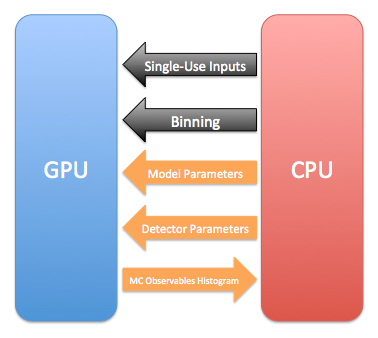
\includegraphics[width=0.6\textwidth]{gpu_usage}
	\caption{The memory flow in the Monte Carlo Matching Framework.  The black arrows represent memory transfers that are performed a single time while orange arrows represent memory transfers that are performed in each log-likelihood calculation.}
	\label{fig:gpu_usage}
\end{figure}




%The GPU framework used for the analyses described in this work can essentially be broken down into two stages: the Monte Carlo simulation and sorting simulated events into histograms.  The actual code for both of these stages can be written in CUDA C and using the libraries included in the CUDA computing platform --- both of which are specifically designed by NVIDIA for easy use with their GPUs.


%CUDA comes preloaded with many random number generators in the cuRAND library, including the normal, uniform, and Poisson distributions.  One can easily build short functions using these distributions to create generators for other required distributions such as the binomial and exponential distributions.  CUDA also comes loaded with an extensive library of mathematical functions if those are also required in a simulation.  


%CUDA does not, however, come preloaded with the ability to produce histograms.  However, basic functions to provide this capability can easily be written by the user and utilized.  



%\subsection{Communicating Between CPU and GPU}
%\label{sec:gpu_cpu_communication}



\subsection{Speed Gains for GPUs versus CPU}


While the speed increase for the Monte Carlo varies on the content and the type of CPU and GPU used, in each of our applications we saw speed increases of roughly 100--1000 times on the GPUs used versus the CPUs when performing the Monte Carlo simulation and filling histograms.  This easily pulls otherwise unfeasible tasks into the realm of possibility.


\subsection{Parallelizing GPUs}


Due to the high level of computing power needed to perform the parameter estimation for the neriX nuclear recoil response measurement, we found that the speed increase seen with a single GPU was not quite enough for our purposes.  Therefore we built a custom GPU-based server that could hold and use eight GPU cards at a time.  This server was filled with six GTX 1080 cards from NVIDIA \cite{nvidia_gtx_manual} for a maximum speed of roughly 54 TFLOPs\footnote{A typical CPU falls in the range of tens to hundreds of GFLOPs.}.  A photo of the GPU server mounted and in use is shown in \figref{fig:gpu_server}.

\begin{figure}[t]
        \centering
	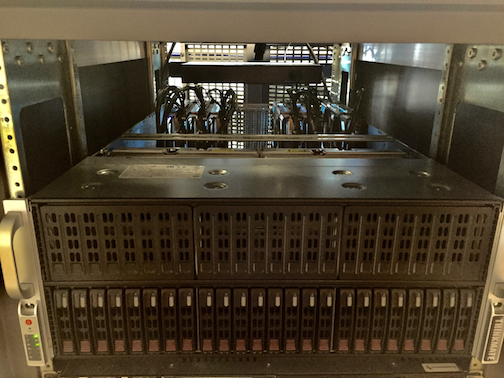
\includegraphics[width=0.6\textwidth]{gpu_server}
	\caption{The GPU-based server used for the analyses in this work.  The actual GPU cards can be seen towards the back of the server (three on the left and right sides).}
	\label{fig:gpu_server}
\end{figure}


The parallelization model that proved the most efficienct also proved to be the simplest.  Each GPU card was activated and managed by a single CPU thread.  The MCMC used for each fit utilized the affine-invariant algorithm \cite{foreman2013emcee} that requires multiple ``walkers'' calculating the log-likelihood at different positions in the parameter space at each step\footnote{In all analyses in this work, either 256 or 512 walkers were used to sample the posterior.}.  Therefore, a first-in-first-out queue data structure was used to pass the parameters of the fit of each walker to each CPU thread which in turn used its individual GPU card to run the Monte Carlo simulation and sorting for the log-likelihood calculation.  We found that this implementation had negligible efficiency losses so the speed of parameter estimation increased linearly with the number of GPU cards used.


\section{Discussion}


GPU-based Monte Carlo matching methods open the door to many exciting possibilities --- all of the major analyses discussed in this work, including the electronic and nuclear recoil calibrations of XENON1T, the nuclear recoil response measurement of neriX, and the characterization of the single photoelectron response of PMTs, were only made possible through the methods discussed in this appendix.  While other methods have been used to perform these measurements, they typically involved large simplifications.  With GPUs, however, our models can be significantly more complicated than they could have been in the past.  Even more exciting is that GPU technology is rapidly improving every year and each new card introduced is a significant improvement on the previous generation so the gains are only likely to improve.

Since the GPU code is very specific to the application, individual examples have not been included in this appendix.  However, all of the author's work and countless examples from other sources are publicly available for reference online.




